\documentclass[../../../main.tex]{subfiles}
\begin{document}

%%%%%%%%%%%%%%%%%%%%%%%%%%%%%%%%%%%%%%%%%
%%%%%%%%%%%%%%%%%%%%%%%%%%%%%%%%%%%%%%%%%
%%%%%%%%%%%%%%%%%%%%%%%%%%%%%%%%%%%%%%%%%
\chapter{Hypothesis testing procedure}

There is a general procedure that we should always follow when performing a hypothesis test. We have already seen it in outline, but now we can be more specific. 


%%%%%%%%%%%%%%%%%%%%%%%%%%%%%%%%%%%%%%%%%
%%%%%%%%%%%%%%%%%%%%%%%%%%%%%%%%%%%%%%%%%
\section{The procedure}

To perform a hypothesis test (with one sample), the procedure we should follow always runs like this: 

\begin{enumerate}

  \item Establish the null and alternative hypotheses. 
  \item Decide if you need to use the z-curve or t-curve.
  \item Decide on an $\alpha$ value.
  \item State your decision rule.
  \item Take a sample.
  \item Compute the mean and STDEV for your sample.
  \item Calculate the z (or t) score for the mean of your sample.
  \item Compare the calculated z (or t) score to your decision rule, and make a decision.
  \item State your results.

\end{enumerate}

\noindent
To flesh out each step, let's walk through the procedure with some examples.


%%%%%%%%%%%%%%%%%%%%%%%%%%%%%%%%%%%%%%%%%
%%%%%%%%%%%%%%%%%%%%%%%%%%%%%%%%%%%%%%%%%
\section{Example 1}

Suppose that McCallister Logistics has a very large fleet of Peterbilt 18-wheelers, which they use to haul various goods around the country. At one point in time, McCallister had established that their trucks consumed fuel at an average rate of 6.2 mpg (miles per gallon), with a standard deviation of 0.2. Earlier this year, McCallister outfit the entire fleet with a new type of tire, because that particular type of tire (or so the maker of the tire claims) is guaranteed to improve fuel efficiency. To figure out if this is true, McCallister randomly selected 40 different trucks and collected each one's fuel efficiency (in miles per gallon). The average for the entire sample turned out to be 6.3 mpg. The company would like us to check if the fuel efficiency improved in a statistically significant way, with a 95\% level of significance. Let us follow our procedure.


%%%%%%%%%%%%%%%%%%%%%%%%%%%%%%%%%%%%%%%%%
\subsection{Establish the test hypotheses}

First, we \vocab{establish the test hypotheses}. The claim by the tire company is that their tire will improve fuel efficiency. This is an implied challenge. So let us assume that the status quo is this: the tire does \emph{not} improve fuel efficiency. Then, the alternative hypothesis will be that the tire \emph{does} improve fuel efficiency.

Let us state the null hypothesis first. We want to say that the tire does not improve fuel efficiency. So, this means that the true population mean will be less than or equal to 6.2mpg. Hence, our null hypothesis is this:

\begin{equation*}
  \NullHyp/: \populationmean \leq 6.2
\end{equation*}

\noindent
The alternative hypothesis must be the opposite:

\begin{equation*}
  \AltHyp/: \populationmean > 6.2
\end{equation*}

\noindent
Is this a two-tailed test, or a one-tailed test (and which direction)? It is a one-tailed test, and in particular it is a right tailed test, because the wedge symbol in the alternative hypothesis points to the right.

We could plot a curve, with the hypothesized mean $\HypPopMean/$ centered at 6.2:

\begin{center}
  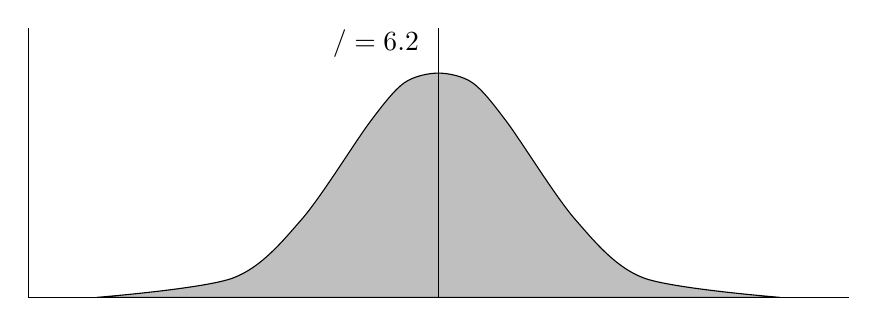
\begin{tikzpicture}
    \begin{axis}[
      axis lines*=left,
      ytick=\empty,
      xtick=\empty,
      height=5cm,
      width=12cm,
      enlarge y limits={value=0.2,upper},
      ]
      \addplot[smooth, fill=lightgray, domain=-10:10] 
        coordinates{
          (-5, 0) (-3, 0.5) (-2, 2) (-1, 4.5) (-0.5, 5.5)
          (0, 5.75)
          (0.5, 5.5) (1, 4.5) (2, 2) (3, 0.5) (5, 0)} 
        \closedcycle;

      \draw (0, 0) -- (0, 8);
      \node at (0, 6.5) [label=left:{$\HypPopMean/ = 6.2$}] {};

    \end{axis}
  \end{tikzpicture}
\end{center}

\noindent
But we actually don't need to draw this graph in terms of mpg. As we perform our test, we will only care about z-scores (or t-scores), which are units of standard deviations. So let us relabel the graph, with units of standard deviations instead of mpgs:

\begin{center}
  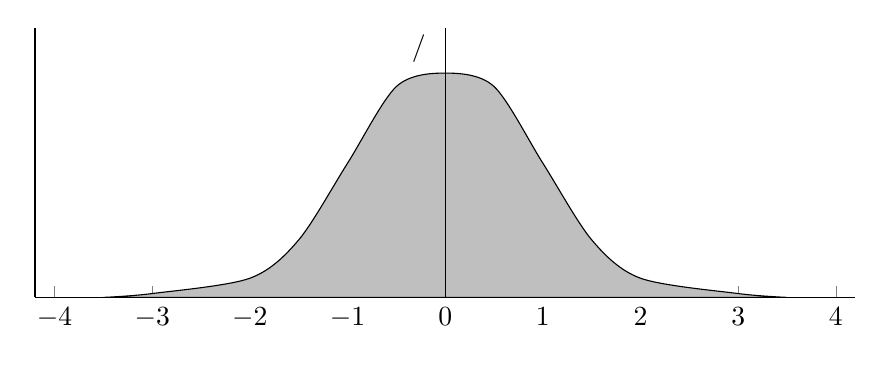
\begin{tikzpicture}
    \begin{axis}[
      axis lines*=left,
      ytick=\empty,
      height=5cm,
      width=12cm,
      enlarge y limits={value=0.2,upper},
      ]
      \addplot[smooth, fill=lightgray, domain=-10:10] 
        coordinates{
          (-3.5, 0) (-3, 0.1) (-2, 0.5) (-1.5, 1.5) (-1, 3.5) (-0.5, 5.5) 
          (0, 5.85)
          (0.5, 5.5) (1, 3.5) (1.5, 1.5) (2, 0.5) (3, 0.1) (3.5, 0)} 
        \closedcycle;

      \draw (0, 0) -- (0, 8);
      \node at (0, 6.5) [label=left:{$\HypPopMean/$}] {};

    \end{axis}
  \end{tikzpicture}
\end{center}


%%%%%%%%%%%%%%%%%%%%%%%%%%%%%%%%%%%%%%%%%
\subsection{Use the z- or t-distribution?}

Next, we need to decide if we should use the \vocab{z- or t-distribution}. The criteria for deciding which one to use are the same as when we calculated confidence intervals. If we know the population standard deviation, or we have a large sample (more than 30 specimens), then we can use the z-distribution. If we don't know the population standard deviation, or if we have a small sample, then we should use the t-distribution.

In this case, we know the population standard deviation, and we have a large enough sample, so we can use the z-distribution.


%%%%%%%%%%%%%%%%%%%%%%%%%%%%%%%%%%%%%%%%%
\subsection{Decide on an $\alpha$ value}

Next we should decide on the \vocab{critical point}. The company has decided already what the $\alpha$ value should be. They told us they want our decision with a 95\% level of significance, so the $\alpha$ value is going to be 5\%, or 0.05.

This is a one-tailed test (on the right), so we're going to put all of $\alpha$ over on the right tail. We're not going to divide it into two parts, and put 2.5\% on the left tail, and 2.5\% on the right tail. We will put all 5\% in the right tail. 

We need to know where exactly to draw the $\alpha$ line though. We know it's 5\% that we want to chop off the right tail, and we know that the z-score for 0.05 is 1.645. Hence, we can draw that on our plot:

\begin{center}
  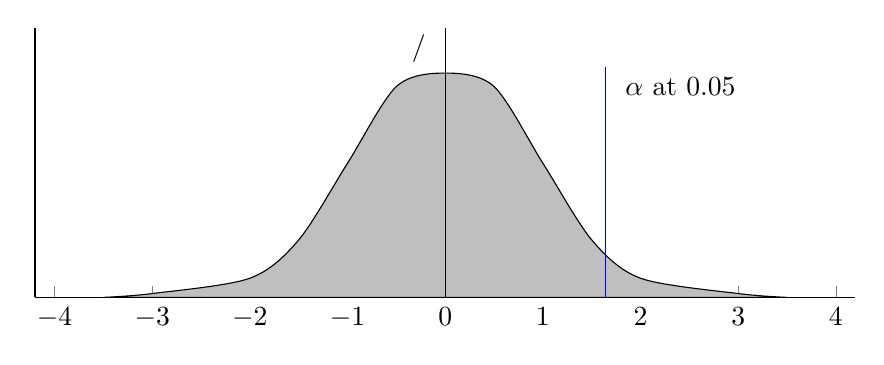
\begin{tikzpicture}
    \begin{axis}[
      axis lines*=left,
      ytick=\empty,
      height=5cm,
      width=12cm,
      enlarge y limits={value=0.2,upper},
      ]
      \addplot[smooth, fill=lightgray, domain=-10:10] 
        coordinates{
          (-3.5, 0) (-3, 0.1) (-2, 0.5) (-1.5, 1.5) (-1, 3.5) (-0.5, 5.5) 
          (0, 5.85)
          (0.5, 5.5) (1, 3.5) (1.5, 1.5) (2, 0.5) (3, 0.1) (3.5, 0)} 
        \closedcycle;

      \draw (0, 0) -- (0, 8);
      \node at (0, 6.5) [label=left:{$\HypPopMean/$}] {};

      \draw[color=blue] (1.645, 0) -- (1.645, 6);
      \node at (1.645, 5.5) [label=right:{$\alpha$ at $0.05$}] {};

    \end{axis}
  \end{tikzpicture}
\end{center}

\noindent
The area of the curve to the right of this line contains exactly 5\% of the total area of the curve. Let's color in the alpha area so it's more visible:

\begin{center}
  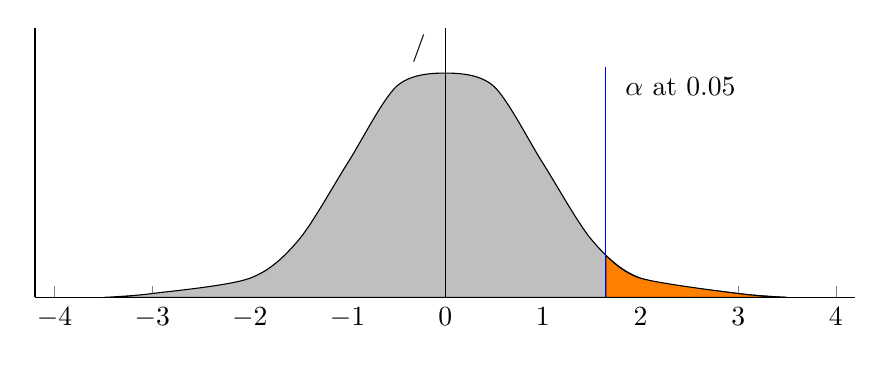
\begin{tikzpicture}
    \begin{axis}[
      axis lines*=left,
      ytick=\empty,
      height=5cm,
      width=12cm,
      enlarge y limits={value=0.2,upper},
      ]
      \addplot[smooth, fill=lightgray, domain=-10:10] 
        coordinates{
          (-3.5, 0) (-3, 0.1) (-2, 0.5) (-1.5, 1.5) (-1, 3.5) (-0.5, 5.5) 
          (0, 5.85)
          (0.5, 5.5) (1, 3.5) (1.5, 1.5) (2, 0.5) (3, 0.1) (3.5, 0)} 
        \closedcycle;

      \addplot[smooth, fill=orange, domain=-10:10] 
        coordinates{
          (1.645, 1.1) (2, 0.5) (3, 0.1) (3.5, 0)} 
        \closedcycle;

      \draw (0, 0) -- (0, 8);
      \node at (0, 6.5) [label=left:{$\HypPopMean/$}] {};

      \draw[color=blue] (1.645, 0) -- (1.645, 6);
      \node at (1.645, 5.5) [label=right:{$\alpha$ at $0.05$}] {};

    \end{axis}
  \end{tikzpicture}
\end{center}

\noindent
At this point, we have successfully set our critical point. Sometimes this is written as $Z_{\alpha}$. So we could write this if we wanted:

\begin{equation*}
  Z_{\alpha} = 1.645
\end{equation*}

\noindent
In fact, let's label the line with that value:

\begin{center}
  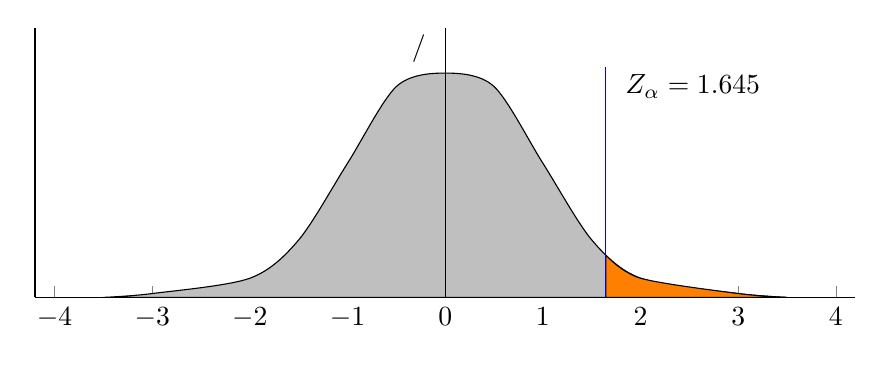
\begin{tikzpicture}
    \begin{axis}[
      axis lines*=left,
      ytick=\empty,
      height=5cm,
      width=12cm,
      enlarge y limits={value=0.2,upper},
      ]
      \addplot[smooth, fill=lightgray, domain=-10:10] 
        coordinates{
          (-3.5, 0) (-3, 0.1) (-2, 0.5) (-1.5, 1.5) (-1, 3.5) (-0.5, 5.5) 
          (0, 5.85)
          (0.5, 5.5) (1, 3.5) (1.5, 1.5) (2, 0.5) (3, 0.1) (3.5, 0)} 
        \closedcycle;

      \addplot[smooth, fill=orange, domain=-10:10] 
        coordinates{
          (1.645, 1.1) (2, 0.5) (3, 0.1) (3.5, 0)} 
        \closedcycle;

      \draw (0, 0) -- (0, 8);
      \node at (0, 6.5) [label=left:{$\HypPopMean/$}] {};

      \draw[color=blue] (1.645, 0) -- (1.645, 6);
      \node at (1.645, 5.5) [label=right:{$Z_{\alpha} = 1.645$}] {};

    \end{axis}
  \end{tikzpicture}
\end{center}


%%%%%%%%%%%%%%%%%%%%%%%%%%%%%%%%%%%%%%%%%
\subsection{State the decision rule}

Now we need to state our \vocab{decision rule}. A decision rule tells us under what conditions we should reject the null hypothesis, and under what conditions we should not reject it.

In this case, we are running a right-tailed test, which says that if we want to overturn the null hypothesis, we need a sample mean that is large enough to convince us that the true population mean is over to the right. 

To check this, we will calculate the z-score for the sample mean, so that we know how many standard deviations from the mean the sample mean falls on our plot. As noted already, the z-score for the sample mean that we will compute is called the \vocab{test statistic}, or the \vocab{calculated z-score}, and it is often written as $Z_{c}$.

So, our decision rule is going to say this: we will reject the null hypothesis if we get a test statistic that is larger than (farther to the right of) the critical point, otherwise the null hypothesis will stand. So here's the rule:

\begin{align*}
  \text{reject } \NullHyp/: \text{ if } Z_{c} > Z_{\alpha} \\
  \text{accept } \NullHyp/: \text{ if } Z_{c} \leq Z_{\alpha}
\end{align*}

\noindent
That is to say, if we take a sample, and the mean of that sample falls to the right of the critical point, then that counts as strong enough evidence to persuade us to reject the null hypothesis. After all, if we get a sample mean that is indeed that far to the right, then that would strongly suggest that the sample came not from the $\HypPopMean/$ population, but rather from another population that is farther to the right.

Conversely, if we take a sample and the mean of that sample falls to the left of the critical point, then we do not have enough evidence to overturn the null hypothesis. 

In our case, the critical point $Z_{\alpha}$ is 1.645, so we can state our decision rule like this:

\begin{align*}
  \text{reject } \NullHyp/: \text{ if } Z_{c} > 1.645 \\
  \text{accept } \NullHyp/: \text{ if } Z_{c} \leq 1.645
\end{align*}


%%%%%%%%%%%%%%%%%%%%%%%%%%%%%%%%%%%%%%%%%
\subsection{Take a sample}

Next, we would \vocab{take a sample} and collect our measurements, but in this case, McCallister has already done that for us. So we know already that our sample has a size of 40 (McCallister randomly selected 40 trucks).


%%%%%%%%%%%%%%%%%%%%%%%%%%%%%%%%%%%%%%%%%
\subsection{Compute the mean and STDEV}

We would also calculate the \vocab{mean} and \vocab{standard deviation} for our sample. In this case, McCallister already did that. After collecting the fuel efficiency (in miles per gallon) for each truck, McCallister found that the mean of those 40 trucks was 6.3.

We do not need to calculate a standard deviation for this sample, because we know the standard deviation of the population, which is 0.2. We only really need to compute the standard deviation of the sample when we do not know the population standard deviation.


%%%%%%%%%%%%%%%%%%%%%%%%%%%%%%%%%%%%%%%%%
\subsection{Calculate the z-score for the sample mean}

Next, we want to calculate the \vocab{z-score} for the mean of our sample. The sample mean in this case is 6.3. We can compute the z-score for this by using the formula from above, like so:

\begin{equation*}
  Z_{c} = \frac{\samplemean{x} - \HypPopMean/}{\frac{\populationstdev}{\sqrt{\samplesize/}}} = \frac{6.3 - 6.2}{\frac{0.2}{\sqrt{40}}} = 3.16
\end{equation*}

\noindent
So the calculated z-score for the sample mean of 6.3 is 3.16. Let's draw it:

\begin{center}
  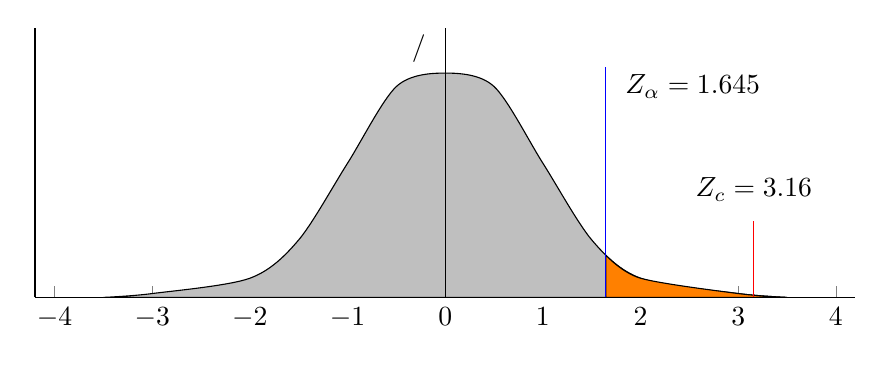
\begin{tikzpicture}
    \begin{axis}[
      axis lines*=left,
      ytick=\empty,
      height=5cm,
      width=12cm,
      enlarge y limits={value=0.2,upper},
      ]
      \addplot[smooth, fill=lightgray, domain=-10:10] 
        coordinates{
          (-3.5, 0) (-3, 0.1) (-2, 0.5) (-1.5, 1.5) (-1, 3.5) (-0.5, 5.5) 
          (0, 5.85)
          (0.5, 5.5) (1, 3.5) (1.5, 1.5) (2, 0.5) (3, 0.1) (3.5, 0)} 
        \closedcycle;

      \addplot[smooth, fill=orange, domain=-10:10] 
        coordinates{
          (1.645, 1.1) (2, 0.5) (3, 0.1) (3.5, 0)} 
        \closedcycle;

      \draw (0, 0) -- (0, 8);
      \node at (0, 6.5) [label=left:{$\HypPopMean/$}] {};

      \draw[color=blue] (1.645, 0) -- (1.645, 6);
      \node at (1.645, 5.5) [label=right:{$Z_{\alpha} = 1.645$}] {};

      \draw[color=red] (3.16, 0) -- (3.16, 2);
      \node at (3.16, 2) [label=above:{$Z_{c} = 3.16$}] {};

    \end{axis}
  \end{tikzpicture}
\end{center}


%%%%%%%%%%%%%%%%%%%%%%%%%%%%%%%%%%%%%%%%%
\subsection{Use the decision rule to make a decision}

Now we \vocab{use the decision rule} to decide if our sample provides enough evidence to overturn the null hypothesis. Our decision rule was this:

\begin{align*}
  \text{reject } \NullHyp/: \text{ if } Z_{c} > 1.645 \\
  \text{accept } \NullHyp/: \text{ if } Z_{c} \leq 1.645
\end{align*}

\noindent
So we will reject the null hypothesis if our test statistic is greater than 1.645. Our test statistic is 3.16, which is indeed greater than 1.645, so we can reject the null hypothesis. This sample has a mean that is over 3 standard deviations from the hypothesized mean, so it very likely comes from another population over on the right.


%%%%%%%%%%%%%%%%%%%%%%%%%%%%%%%%%%%%%%%%%
\subsection{State the result}

Now we can \vocab{state the result}. If we want to put this formally, we can say this:

\begin{quote}
  With a 95\% level of significance, we cannot accept the null hypothesis that the population mean is less than or equal to 6.2 mpg.
\end{quote}

\noindent
More informally, we could report to McCallister:

\begin{quote}
  Yep, you're getting better gas mileage.
\end{quote}



%%%%%%%%%%%%%%%%%%%%%%%%%%%%%%%%%%%%%%%%%
%%%%%%%%%%%%%%%%%%%%%%%%%%%%%%%%%%%%%%%%%
\section{Example 2}

VitaZ (pronounce "Vight-ah-Zee") is a company that manufactures and bottles vitamins for other large health companies. A particular brand is supposed to have 100 vitamins per bottle, but some customers have complained that some bottles have less. After some investigation, VitaZ zeros in on one particular bottling machine. They wonder if this particular machine is defective. They want to know if this machine fills bottles with (on average) 100 vitamins, with a 99\% level of significance. The company is concerned that the machine neither underfills nor overfills. As a sample, we are given 10 randomly selected bottles filled by the machine in question. We count the vitamins in each bottle and get the following counts:

\begin{center}
  100, 100, 98, 97, 93, 101, 98, 100, 99, 96
\end{center}


%%%%%%%%%%%%%%%%%%%%%%%%%%%%%%%%%%%%%%%%%
\subsection{Establish the test hypotheses}

The first step is to \vocab{establish the test hypotheses}. The company wants to know that the mean vitamin count is 100, rather than more or less. Since they want to know that the mean does not stray higher or lower than 100, that tells us this is a two-tailed test.

The hypotheses for a two-tailed test have this form:

\begin{align*}
  \NullHyp/: \populationmean = \HypPopMean/ \\
  \AltHyp/: \populationmean \not = \HypPopMean/ 
\end{align*}

\noindent
In this case, the hypothesized population mean $\HypPopMean/$ is 100, and so the null hypothesis will be that the true population mean is the same as that:

\begin{equation*}
  \NullHyp/: \populationmean = 100
\end{equation*}

\noindent
And the alternative hypothesis will be that the true population mean is not 100:

\begin{equation*}
  \AltHyp/: \populationmean \not = 100
\end{equation*}

\noindent
Note the hypothesized population mean $\HypPopMean/$ is 100.

%%%%%%%%%%%%%%%%%%%%%%%%%%%%%%%%%%%%%%%%%
\subsection{Use the z- or t-distribution?}

Next we determine if we should use the \vocab{z- or t-distribution}. Which should we use? We should use a z-distribution for a large sample (30 or more specimens) or if we know the population standard deviation. We do not know the population standard deviation, and we do not have a large sample size, so we will use the t-distribution.

The sample size $\samplesize/$ is 10, so the degrees of freedom is $\samplesize/ - 1 = 9$. Hence, we will use the t-distribution with 9 degrees of freedom. We can plot it:

\begin{center}
  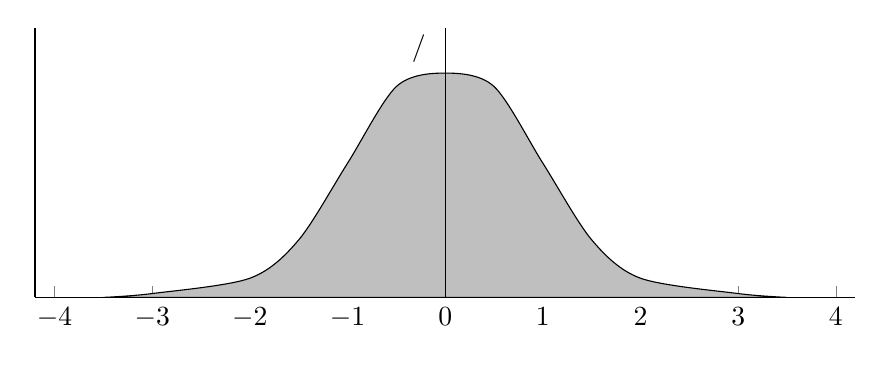
\begin{tikzpicture}
    \begin{axis}[
      axis lines*=left,
      ytick=\empty,
      height=5cm,
      width=12cm,
      enlarge y limits={value=0.2,upper},
      ]
      \addplot[smooth, fill=lightgray, domain=-10:10] 
        coordinates{
          (-3.5, 0) (-3, 0.1) (-2, 0.5) (-1.5, 1.5) (-1, 3.5) (-0.5, 5.5) 
          (0, 5.85)
          (0.5, 5.5) (1, 3.5) (1.5, 1.5) (2, 0.5) (3, 0.1) (3.5, 0)} 
        \closedcycle;

      \draw (0, 0) -- (0, 8);
      \node at (0, 6.5) [label=left:{$\HypPopMean/$}] {};

    \end{axis}
  \end{tikzpicture}
\end{center}


%%%%%%%%%%%%%%%%%%%%%%%%%%%%%%%%%%%%%%%%%
\subsection{Decide on an $\alpha$ value}

Next, we should \vocab{set our critical value(s)}. Where should our critical value(s) be? The VitaZ company has said they want a confidence level of 99\%, so our $\alpha$ area will be 1\%, or 0.01. However, this is a two-tailed test, so we need to divide that into two, and put half in each tail (i.e., 0.005 in each):

\begin{center}
  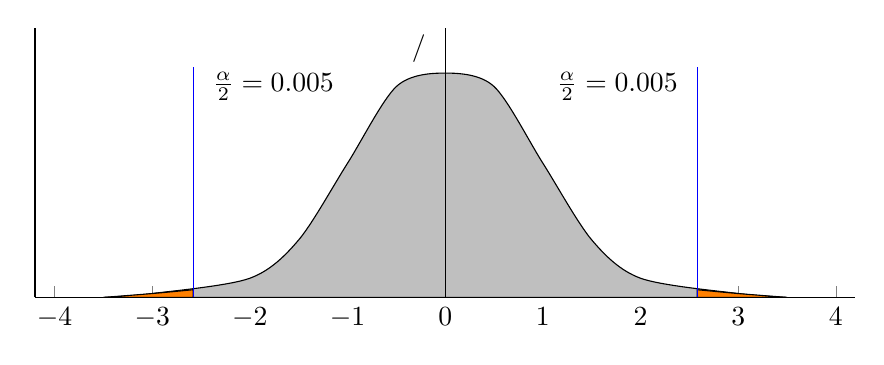
\begin{tikzpicture}
    \begin{axis}[
      axis lines*=left,
      ytick=\empty,
      height=5cm,
      width=12cm,
      enlarge y limits={value=0.2,upper},
      ]
      \addplot[smooth, fill=lightgray, domain=-10:10] 
        coordinates{
          (-3.5, 0) (-3, 0.1) (-2, 0.5) (-1.5, 1.5) (-1, 3.5) (-0.5, 5.5) 
          (0, 5.85)
          (0.5, 5.5) (1, 3.5) (1.5, 1.5) (2, 0.5) (3, 0.1) (3.5, 0)} 
        \closedcycle;

      \addplot[smooth, fill=orange, domain=-10:10] 
        coordinates{(-3.5, 0) (-3, 0.1) (-2.58, 0.2)} 
        \closedcycle;

      \addplot[smooth, fill=orange, domain=-10:10] 
        coordinates{(2.58, 0.2) (3, 0.1) (3.5, 0)} 
        \closedcycle;

      \draw (0, 0) -- (0, 8);
      \node at (0, 6.5) [label=left:{$\HypPopMean/$}] {};

      \draw[color=blue] (-2.58, 0) -- (-2.58, 6);
      \node at (-2.58, 5.5) [label=right:{$\frac{\alpha}{2} = 0.005$}] {};

      \draw[color=blue] (2.58, 0) -- (2.58, 6);
      \node at (2.58, 5.5) [label=left:{$\frac{\alpha}{2} = 0.005$}] {};

    \end{axis}
  \end{tikzpicture}
\end{center}

\noindent
With a z-distribution, we call the critical point $Z_{\alpha}$, or if it's divided into two, we label each one $Z_{\frac{\alpha}{2}}$. With a t-distribution, we can write it as $t_{\alpha}$, or if it's divided into two, we can label it as $t_{\frac{\alpha}{2}}$. What are the t-values for 0.005? They are 2.58 standard deviations on either side of the mean. Hence, $t_{\frac{\alpha}{2}} = \pm 2.58$:

\begin{center}
  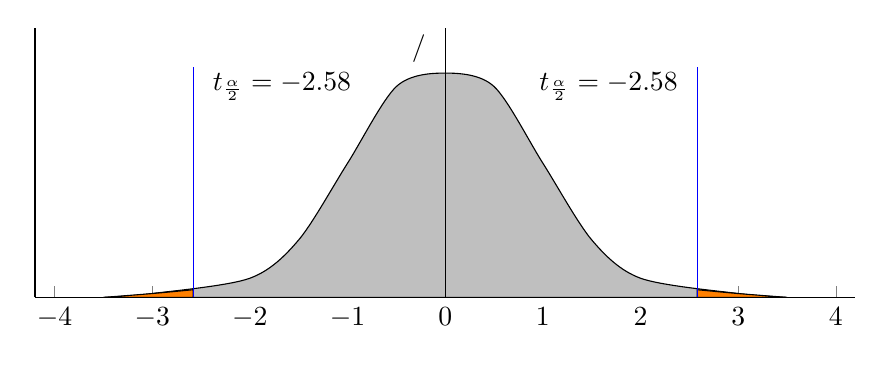
\begin{tikzpicture}
    \begin{axis}[
      axis lines*=left,
      ytick=\empty,
      height=5cm,
      width=12cm,
      enlarge y limits={value=0.2,upper},
      ]
      \addplot[smooth, fill=lightgray, domain=-10:10] 
        coordinates{
          (-3.5, 0) (-3, 0.1) (-2, 0.5) (-1.5, 1.5) (-1, 3.5) (-0.5, 5.5) 
          (0, 5.85)
          (0.5, 5.5) (1, 3.5) (1.5, 1.5) (2, 0.5) (3, 0.1) (3.5, 0)} 
        \closedcycle;

      \addplot[smooth, fill=orange, domain=-10:10] 
        coordinates{(-3.5, 0) (-3, 0.1) (-2.58, 0.2)} 
        \closedcycle;

      \addplot[smooth, fill=orange, domain=-10:10] 
        coordinates{(2.58, 0.2) (3, 0.1) (3.5, 0)} 
        \closedcycle;

      \draw (0, 0) -- (0, 8);
      \node at (0, 6.5) [label=left:{$\HypPopMean/$}] {};

      \draw[color=blue] (-2.58, 0) -- (-2.58, 6);
      \node at (-2.58, 5.5) [label=right:{$t_{\frac{\alpha}{2}} = -2.58$}] {};

      \draw[color=blue] (2.58, 0) -- (2.58, 6);
      \node at (2.58, 5.5) [label=left:{$t_{\frac{\alpha}{2}} = -2.58$}] {};

    \end{axis}
  \end{tikzpicture}
\end{center}


%%%%%%%%%%%%%%%%%%%%%%%%%%%%%%%%%%%%%%%%%
\subsection{State the decision rule}

Next, we must \vocab{state our decision rule}. In this case, as in all two-tailed tests, we won't reject the null hypothesis if we get a sample mean that falls anywhere in the grey region. That is to say, any sample mean that falls between the two $t_{\frac{\alpha}{2}}$ lines is likely a sample that comes from the population centered at $\HypPopMean/$. So we won't reject the null hypothesis if we get a sample mean that falls there.

By contrast, if we get a sample mean that falls outside the two $t_{\frac{\alpha}{2}}$ lines, then it is very likely that such a sample comes from another population farther out. It \emph{could} be a sample that comes from the hypothesized mean $\HypPopMean/$, but there is only a half percent (0.005) chance of that. It's much more likely that the true population mean is farther out, and the sample we get comes from that. So, we will reject the null hypothesis if we get a sample mean outside the two $t_{\frac{\alpha}{2}}$ lines.

Let us state the rule. When we take the sample mean, we will calculate the t-score for that mean. We call this the \vocab{calculated t-score} or the \vocab{test statistic} (much like how it is called the \vocab{calculated z-score} if we are using the z-distribution). For our rule, we want to say that we will reject the null hypothesis only if the test statistic falls outside the two critical points at $t_{\frac{\alpha}{2}}$.

The general decision rule for a two-tailed test is thus:

\begin{align*}
  \text{reject } \NullHyp/: \text{ if } t_{c} < -t_{\frac{\alpha}{2}} \text{ or } t_{c} > t_{\frac{\alpha}{2}} \\
  \text{accept } \NullHyp/: \text{ if } t_{c} > -t_{\frac{\alpha}{2}} \text{ and } t_{c} < t_{\frac{\alpha}{2}}
\end{align*}

\noindent
We can plug in our $t_{\frac{\alpha}{2}}$ values (-2.58 and +2.58), and we get this:

\begin{align*}
  \text{reject } \NullHyp/: \text{ if } t_{c} < -2.58 \text{ or } t_{c} > 2.58 \\
  \text{accept } \NullHyp/: \text{ if } t_{c} > -2.58 \text{ and } t_{c} < 2.58
\end{align*}


%%%%%%%%%%%%%%%%%%%%%%%%%%%%%%%%%%%%%%%%%
\subsection{Take a sample}

If we haven't already got a sample, we would now proceed to \vocab{collect a sample} and collect our measurements. In this case, we already have the sample of 10 bottles, with the vitamin counts in each one.


%%%%%%%%%%%%%%%%%%%%%%%%%%%%%%%%%%%%%%%%%
\subsection{Compute the mean and STDEV}

We need to \vocab{compute the mean and STDEV} of the sample. First, the mean. To compute the mean, we add all the values, and divide by the sample size:

\begin{equation*}
  \samplemean{x} = \frac{100 + 100 + 98 + 97 + 93 + 101 + 98 + 100 + 99 + 96}{10} = 98.2
\end{equation*}

\noindent
To calculate the standard deviation $\samplestdev$, we first compute the variance $\samplevariance$. To do this, for each value in our sample we calculate its deviation (how far it is from the mean) and then we square it:

\begin{align*}
  (100 - 98.2)^{2} = 3.24 \hskip 1cm (100 - 98.2)^{2} = 3.24 \\
  (98 - 98.2)^{2} = 0.04 \hskip 1cm (97 - 98.2)^{2} = 1.44 \\
  (93 - 98.2)^{2} = 27.04 \hskip 1cm (101 - 98.2)^{2} = 7.84 \\
  (100 - 98.2)^{2} = 3.24 \hskip 1cm (98 - 98.2)^{2} = 0.04 \\
  (99 - 98.2)^{2} = 0.64 \hskip 1cm (96 - 98.2)^{2} =  4.84
\end{align*}

\noindent
Then we take the average (mean) of all those values:

\begin{equation*}
  \samplevariance = \frac{3.24 + 3.24 + 0.04 + 1.44 + 27.04 + 7.84 + 3.24 + 0.04 + 0.64 + 4.84}{10} = 5.16
\end{equation*}

\noindent
And finally, to find the STDEV of our sample, we take the square root of the variance:

\begin{equation*}
  \samplestdev = \sqrt{\samplevariance} = \sqrt{5.16} = 2.27
\end{equation*}


%%%%%%%%%%%%%%%%%%%%%%%%%%%%%%%%%%%%%%%%%
\subsection{Calculate the t-score for the sample mean}

Next, we \vocab{calculate the t-score} (our test statistic) for the sample mean (98.2). The formula to calculate a t-score for a sample distribution is:

\begin{equation*}
  t_{c} = \frac{\samplemean{x} - \HypPopMean/}{\frac{\samplestdev}{\sqrt{\samplesize/}}}
\end{equation*}

\noindent
Then if we substitute in our values:

\begin{equation*}
  t_{c} = \frac{98.2 - 98}{\frac{2.27}{\sqrt{10}}} = 0.28
\end{equation*}

\noindent
So, the sample mean of 0.28 falls 0.28 standard deviations away from the center of the hypothesized sampling distribution. Let's draw it on the plot:

\begin{center}
  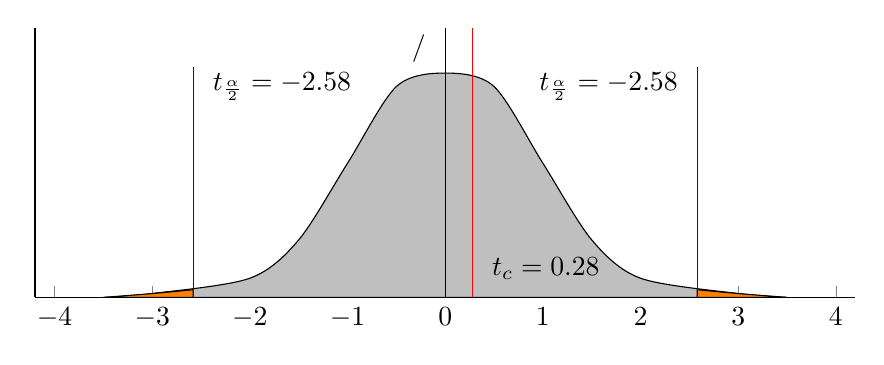
\begin{tikzpicture}
    \begin{axis}[
      axis lines*=left,
      ytick=\empty,
      height=5cm,
      width=12cm,
      enlarge y limits={value=0.2,upper},
      ]
      \addplot[smooth, fill=lightgray, domain=-10:10] 
        coordinates{
          (-3.5, 0) (-3, 0.1) (-2, 0.5) (-1.5, 1.5) (-1, 3.5) (-0.5, 5.5) 
          (0, 5.85)
          (0.5, 5.5) (1, 3.5) (1.5, 1.5) (2, 0.5) (3, 0.1) (3.5, 0)} 
        \closedcycle;

      \addplot[smooth, fill=orange, domain=-10:10] 
        coordinates{(-3.5, 0) (-3, 0.1) (-2.58, 0.2)} 
        \closedcycle;

      \addplot[smooth, fill=orange, domain=-10:10] 
        coordinates{(2.58, 0.2) (3, 0.1) (3.5, 0)} 
        \closedcycle;

      \draw (0, 0) -- (0, 8);
      \node at (0, 6.5) [label=left:{$\HypPopMean/$}] {};

      \draw[color=blue] (-2.58, 0) -- (-2.58, 6);
      \node at (-2.58, 5.5) [label=right:{$t_{\frac{\alpha}{2}} = -2.58$}] {};

      \draw[color=blue] (2.58, 0) -- (2.58, 6);
      \node at (2.58, 5.5) [label=left:{$t_{\frac{\alpha}{2}} = -2.58$}] {};

      \draw[color=red] (0.28, 0) -- (0.28, 10);
      \node at (0.28, 0.75) [label=right:{$t_{c} = 0.28$}] {};

    \end{axis}
  \end{tikzpicture}
\end{center}


%%%%%%%%%%%%%%%%%%%%%%%%%%%%%%%%%%%%%%%%%
\subsection{Use the decision rule to make a decision}

Now we \vocab{use the decision rule} to decide if our sample provides enough evidence to overturn the null hypothesis. Our decision rule was this:

\begin{align*}
  \text{reject } \NullHyp/: \text{ if } t_{c} < -2.58 \text{ or } t_{c} > 2.58 \\
  \text{accept } \NullHyp/: \text{ if } t_{c} > -2.58 \text{ and } t_{c} < 2.58
\end{align*}

\noindent
This says we will reject the null hypothesis if our test statistic falls outside the two critical points. Our test statistic is 0.28, which does not fall outside our two critical points. On the contrary, it falls in between them. In fact, as we can see in the plot, our test statistic falls very close to the hypothesized mean $\HypPopMean/$. So it is very likely that this sample comes from a population that, if it is not $\HypPopMean/$ itself, is very close to it. Hence, we do not have strong enough evidence to overturn the null hypothesis.


%%%%%%%%%%%%%%%%%%%%%%%%%%%%%%%%%%%%%%%%%
\subsection{State the result}

Now we can \vocab{state the result}. Formally, we can say:

\begin{quote}
  With a 99\% level of significance, we cannot reject the null hypothesis that the population mean is 100 vitamins per bottle.
\end{quote}

\noindent
More informally, we can report to VitaZ:

\begin{quote}
  The sample does not provide enough evidence to suggest that the machine is defective.
\end{quote}



\end{document}
